%%%%%%%%%%%%%%%%%%%%%%%%%%%%%%%%%%%%%%%%%
% The Legrand Orange Book
% LaTeX Template
% Version 3.1 (February 18, 2022)
%
% This template originates from:
% https://www.LaTeXTemplates.com
%
% Authors:
% Vel (vel@latextemplates.com)
% Mathias Legrand (legrand.mathias@gmail.com)
%
% License:
% CC BY-NC-SA 4.0 (https://creativecommons.org/licenses/by-nc-sa/4.0/)
%
% Compiling this template:
% This template uses biber for its bibliography and makeindex for its index.
% When you first open the template, compile it from the command line with the 
% commands below to make sure your LaTeX distribution is configured correctly:
%
% 1) pdflatex main
% 2) makeindex main.idx -s indexstyle.ist
% 3) biber main
% 4) pdflatex main x 2
%
% After this, when you wish to update the bibliography/index use the appropriate
% command above and make sure to compile with pdflatex several times 
% afterwards to propagate your changes to the document.
%
%%%%%%%%%%%%%%%%%%%%%%%%%%%%%%%%%%%%%%%%%

%----------------------------------------------------------------------------------------
%	PACKAGES AND OTHER DOCUMENT CONFIGURATIONS
%----------------------------------------------------------------------------------------

\documentclass[
	11pt, % Default font size, select one of 10pt, 11pt or 12pt
	fleqn, % Left align equations
	a4paper, % Paper size, use either 'a4paper' for A4 size or 'letterpaper' for US letter size
	%oneside, % Uncomment for oneside mode, this doesn't start new chapters and parts on odd pages (adding an empty page if required), this mode is more suitable if the book is to be read on a screen instead of printed
]{LegrandOrangeBook}

% Book information for PDF metadata, remove/comment this block if not required 
\hypersetup{
	pdftitle={Title}, % Title field
	pdfauthor={Author}, % Author field
	pdfsubject={Subject}, % Subject field
	pdfkeywords={Keyword1, Keyword2, ...}, % Keywords
	pdfcreator={LaTeX}, % Content creator field
}

\addbibresource{sample.bib} % Bibliography file

\definecolor{ocre}{RGB}{243, 102, 25} % Define the color used for highlighting throughout the book
% \definecolor{ocre}{RGB}{0, 0, 0} % Define the color used for highlighting throughout the book

\chapterimage{orange1.jpg} % Chapter heading image
\chapterspaceabove{6.5cm} % Default whitespace from the top of the page to the chapter title on chapter pages
\chapterspacebelow{6.75cm} % Default amount of vertical whitespace from the top margin to the start of the text on chapter pages

%----------------------------------------------------------------------------------------

% ******** Eye Protection ********
\usepackage{xcolor} % For defining and using colors
\definecolor{mygreen}{RGB}{205, 222, 194} % Define a custom green color for eye protection
% \pagecolor{mygreen} % Set page background color to custom green
% *******************************

\usepackage[utf8]{inputenc}
\usepackage[T1]{fontenc}
\usepackage{amsmath}
\usepackage{amsfonts}
\usepackage{amssymb}
\usepackage[version=4]{mhchem}
\usepackage{stmaryrd}






\begin{document}

%----------------------------------------------------------------------------------------
%	TITLE PAGE
%----------------------------------------------------------------------------------------

\titlepage % Output the title page
	{
\includegraphics[width=\paperwidth]{background.pdf}} % Code to output the background image, which should be the same dimensions as the paper to fill the page entirely; leave empty for no background image
	{ % Title(s) and author(s)
		\centering\sffamily % Font styling
		{\Huge\bfseries
        Quantum Computation and Optimization
        \par} % Book title
		\vspace{16pt} % Vertical whitespace
		{\LARGE A Study Note\par} % Subtitle
		\vspace{24pt} % Vertical whitespace
		{\huge\bfseries Zhijian Lai, Jiang Hu, Li He\par} % Author name
	}

% %----------------------------------------------------------------------------------------
% %	COPYRIGHT PAGE
% %----------------------------------------------------------------------------------------

% \thispagestyle{empty} % Suppress headers and footers on this page

% ~\vfill % Push the text down to the bottom of the page

% \noindent Copyright \copyright\ 2022 Goro Akechi\\ % Copyright notice

% \noindent \textsc{Published by Publisher}\\ % Publisher

% \noindent \textsc{\href{https://www.latextemplates.com/template/legrand-orange-book}{book-website.com}}\\ % URL

% \noindent Licensed under the Creative Commons Attribution-NonCommercial 4.0 License (the ``License''). You may not use this file except in compliance with the License. You may obtain a copy of the License at \url{https://creativecommons.org/licenses/by-nc-sa/4.0}. Unless required by applicable law or agreed to in writing, software distributed under the License is distributed on an \textsc{``as is'' basis, without warranties or conditions of any kind}, either express or implied. See the License for the specific language governing permissions and limitations under the License.\\ % License information, replace this with your own license (if any)

% \noindent \textit{First printing, March 2022} % Printing/edition date

%----------------------------------------------------------------------------------------
%	TABLE OF CONTENTS
%----------------------------------------------------------------------------------------

\pagestyle{empty} % Disable headers and footers for the following pages

\tableofcontents % Output the table of contents

% \listoffigures % Output the list of figures, comment or remove this command if not required

% \listoftables % Output the list of tables, comment or remove this command if not required

\pagestyle{fancy} % Enable default headers and footers again

\cleardoublepage % Start the following content on a new page

%----------------------------------------------------------------------------------------
%	SECTIONING EXAMPLES CHAPTER
%----------------------------------------------------------------------------------------

\chapterimage{orange2.jpg} % Chapter heading image
\chapterspaceabove{6.75cm} % Whitespace from the top of the page to the chapter title on chapter pages
\chapterspacebelow{7.25cm} % Amount of vertical whitespace from the top margin to the start of the text on chapter pages

%------------------------------------------------

 

% ==========================  正文开始  ==========================
%----------------------------------------------------------------------------------------
%	PART
%----------------------------------------------------------------------------------------

\part{Notes of NC book}
\chapter{Introduction to quantum mechanics}

A good understanding of quantum mechanics is based upon a solid grasp of linear algebra.

\section{Linear algebra}

%   1.1.1 vector space
    \subsection{vector space}
    The vector space of most interest to us is $\mathbf{C}^{n}$, the space of all $n$-tuples of complex numbers, $\left(z_{1}, \ldots, z_{n}\right)$. The elements of a vector space are called vectors, and we will sometimes use the column matrix notation
$$
\left[\begin{array}{c}
z_{1} \\
\vdots \\
z_{n}
\end{array}\right]
$$
to indicate a vector. For convenience, we use the notation $\left(z_{1}, \ldots, z_{n}\right)$ to denote a column matrix with entries $z_{1}, \ldots, z_{n}$. 

There is an addition operation defined which takes pairs of vectors to other vectors. In $\mathbf{C}^{n}$ the addition operation for vectors is defined by
$$
\left[\begin{array}{c}
z_{1} \\
\vdots \\
z_{n}
\end{array}\right]+\left[\begin{array}{c}
z_{1}^{\prime} \\
\vdots \\
z_{n}^{\prime}
\end{array}\right] \equiv\left[\begin{array}{c}
z_{1}+z_{1}^{\prime} \\
\vdots \\
z_{n}+z_{n}^{\prime}
\end{array}\right]
$$
where the addition operations on the right are just ordinary additions of complex numbers. Furthermore, in a vector space there is a scalar multiplication operation. In $\mathbf{C}^{n}$ this is defined by
$$
z\left[\begin{array}{c}
z_{1} \\
\vdots \\
z_{n}
\end{array}\right] \equiv\left[\begin{array}{c}
z z_{1} \\
\vdots \\
z z_{n}
\end{array}\right]
$$
where $z$ is a scalar, that is, a complex number\footnote{Physicists sometimes refer to complex numbers as $c$-numbers.}, and the multiplications on the right are ordinary multiplication of complex numbers. A vector subspace of a vector space $V$ is a subset $W$ of $V$ such that $W$ is also a vector space, that is, $W$ must be closed under scalar multiplication and addition.

We will use the \textit{standard} notation of quantum mechanics for linear algebraic concepts, see Figure \ref{tab:summary_AL}. For a vector in a vector space is the following:
$$
|\psi\rangle .
$$
The notation $|\cdot\rangle$, called "ket", is used to indicate that the object is a (column) vector, and $\psi$ is a label for the vector. The entire object $|\psi\rangle$ is pronounced  as "ket psi". Any label is valid, although we prefer to use simple labels like $\psi$ and $\varphi$.

\begin{remark} %zero vector $0$ and the special vector $|0\rangle$
    A vector space also contains a special zero vector, which we denote by 0. In $\mathbf{C}^{n}$ the zero element is $0=(0,0, \ldots, 0)$. Note that we do not use the ket notation for the zero vector - it is the only exception we shall make. Because, it is conventional to use the notation $|0\rangle$ to mean some special vector that is not zero vector.
\end{remark}

\begin{table}[]
    \centering
    \begin{tabular}{c|l}
        \hline\hline
        Notation & Description \\
        \hline
        $z^{*}$ & Complex conjugate of the complex number $z$. $(1+i)^{*}=1-i$\\
        $|\psi\rangle$& Vector. Also known as a ket. \\
        $\langle\psi|$& Vector dual to $|\psi\rangle$. Also known as a bra. \\
        $\langle\varphi | \psi\rangle$& Inner product between the vectors $|\varphi\rangle$ and $|\psi\rangle$. \\
        $|\varphi\rangle \otimes|\psi\rangle$& Tensor product of $|\varphi\rangle$ and $|\psi\rangle$. \\
        $|\varphi\rangle|\psi\rangle$& Abbreviated notation for tensor product of $|\varphi\rangle$ and $|\psi\rangle$. \\
        $A^{*}$& Complex conjugate of the $A$ matrix. \\
        $A^{T}$& Transpose of the $A$ matrix. \\
         $A^{\dagger}$& Hermitian conjugate or adjoint of the $A$ matrix, $A^{\dagger}=\left(A^{T}\right)^{*}$. \\
         & $\left[\begin{array}{cc}a & b \\ c & d\end{array}\right]^{\dagger}=\left[\begin{array}{cc}a^{*} & c^{*} \\ b^{*} & d^{*}\end{array}\right]$. \\
        $\langle\varphi|A| \psi\rangle$ & Inner product between $|\varphi\rangle$ and $A|\psi\rangle$. \\
         & Equivalently, inner product between $A^{\dagger}|\varphi\rangle$ and $|\psi\rangle$. \\
        \hline\hline
    \end{tabular}
\caption{Summary of some standard quantum mechanical notation for notions from linear algebra. This style of notation is known as the Dirac notation.}
\label{tab:summary_AL}
\end{table}

%   1.1.2 Bases and linear independence
    \subsection{Bases and linear independence}
    A spanning set for a vector space is a set of vectors $\left|v_{1}\right\rangle, \ldots,\left|v_{n}\right\rangle$ such that any vector $|v\rangle$ in the vector space can be written as a linear combination $|v\rangle=\sum_{i} a_{i}\left|v_{i}\right\rangle$ of vectors in that set. 

\begin{example}
    For example, a spanning set for the vector space $\mathbf{C}^{2}$ is the set
    $$
    \left|v_{1}\right\rangle \equiv\left[\begin{array}{l}
    1 \\
    0
    \end{array}\right] ; \quad\left|v_{2}\right\rangle  \equiv\left[\begin{array}{l}
    0 \\
    1
    \end{array}\right]
  $$
    since any vector
    $$
    |v\rangle=\left[\begin{array}{l}
    a_{1} \\
    a_{2}
    \end{array}\right]
    $$
    in $\mathbf{C}^{2}$ can be written as a linear combination $|v\rangle=a_{1}\left|v_{1}\right\rangle+a_{2}\left|v_{2}\right\rangle$ of the vectors $\left|v_{1}\right\rangle$ and $\left|v_{2}\right\rangle$. We say that the vectors $\left|v_{1}\right\rangle$ and $\left|v_{2}\right\rangle$ span the vector space $\mathbf{C}^{2}$.
\end{example}

Generally, a vector space may have many different spanning sets. 

\begin{example}
A second spanning set for the vector space $\mathbf{C}^{2}$ is the set
$$
\left|v_{1}\right\rangle \equiv \frac{1}{\sqrt{2}}\left[\begin{array}{l}
1 \\
1
\end{array}\right] ; \quad\left|v_{2}\right\rangle \equiv \frac{1}{\sqrt{2}}\left[\begin{array}{r}
1 \\
-1
\end{array}\right]
$$
since an arbitrary vector $|v\rangle=\left(a_{1}, a_{2}\right)$ can be written as a linear combination of $\left|v_{1}\right\rangle$ and $\left|v_{2}\right\rangle$,
$$
|v\rangle=\frac{a_{1}+a_{2}}{\sqrt{2}}\left|v_{1}\right\rangle+\frac{a_{1}-a_{2}}{\sqrt{2}}\left|v_{2}\right\rangle.
$$
\end{example}

A set of non-zero vectors $\left|v_{1}\right\rangle, \ldots,\left|v_{n}\right\rangle$ are linearly dependent if there exists a set of complex numbers $a_{1}, \ldots, a_{n}$ with $a_{i} \neq 0$ for at least one value of $i$, such that
$$
a_{1}\left|v_{1}\right\rangle+a_{2}\left|v_{2}\right\rangle+\cdots+a_{n}\left|v_{n}\right\rangle=0.
$$
A set of vectors is linearly independent if it is not linearly dependent. 

It can be shown that any two sets of linearly independent vectors which span a vector space $V$ contain the same number of elements. We call such a set a basis for $V$. Furthermore, such a basis set always exists. The number of elements in the basis is defined to be the dimension of $V$. In this book we will only be interested in finite dimensional vector spaces. 

% Exercise 2.1: (Linear dependence: example) Show that $(1,-1),(1,2)$ and $(2,1)$ are linearly dependent.

%   1.1.3 Linear operators and matrices
    \subsection{Linear operators and matrices}
    A linear operator between vector spaces $V$ and $W$ is defined to be a function $A$ : $V \rightarrow W$ which is linear in its inputs,
\begin{equation}\label{eq:linear-operator}
A\left(\sum_{i} a_{i}\left|v_{i}\right\rangle\right)=\sum_{i} a_{i} A\left(\left|v_{i}\right\rangle\right).
\end{equation}
Usually we just write $A|v\rangle$ to denote $A(|v\rangle)$. When we say that a linear operator $A$ is defined on a vector space, $V$, we mean that $A$ is a linear operator from $V$ to $V$. 

\begin{example}
    An important linear operator on any vector space $V$ is the identity operator, $I_{V}$, defined by the equation $I_{V}|v\rangle \equiv|v\rangle$ for all vectors $|v\rangle$. Where no chance of confusion arises we drop the subscript $V$ and just write $I$ to denote the identity operator. 
\end{example}

\begin{example}
    Another important linear operator is the zero operator, which we denote 0 . The zero operator maps all vectors to the zero vector, $0|v\rangle \equiv 0$. 
\end{example}

It is clear from (\ref{eq:linear-operator}) that once the action of a linear operator $A$ on a basis (of its domain) is specified, the action of $A$ is completely determined on all inputs. This tells us that, when we want to show that two linear operators $A,B:V \rightarrow W$ are the same, we only need to show that $A |v_{i}\rangle = B|v_{i}\rangle$ holds for all $i$ under an arbitrary basis $\{|v_{i}\rangle\}$ of $V.$

Suppose $V, W$, and $X$ are vector spaces, and $A: V \rightarrow W$ and $B: W \rightarrow X$ are linear operators. Then we use the notation $B A$ to denote the composition of $B$ with $A$, defined by $(B A)(|v\rangle) \equiv B(A(|v\rangle))$. Once again, we write $B A|v\rangle$ as an abbreviation for $(B A)(|v\rangle)$.

The most convenient way to understand linear operators is in terms of their matrix representations. In fact, the linear operator and matrix viewpoints turn out to be completely equivalent. 

\paragraph{Every matrix can be regarded as a linear operator}
To see the connection, it helps to first understand that an $m$ by $n$ complex matrix $A$ with entries $A_{i j}$ is in fact a linear operator sending vectors in the vector space $\mathbf{C}^{n}$ to the vector space $\mathbf{C}^{m}$, under matrix multiplication of the matrix $A$ by a vector in $\mathbf{C}^{n}$. We've seen that matrices can be regarded as linear operators.

\paragraph{Every linear operator can be given a matrix representation}
Suppose $A: V \rightarrow W$ is a linear operator between vector spaces $V$ and $W$. Suppose $\left|v_{1}\right\rangle, \ldots,\left|v_{m}\right\rangle$ is a basis for $V$ and $\left|w_{1}\right\rangle, \ldots,\left|w_{n}\right\rangle$ is a basis for $W$. Then for each $j$ in the range $1, \ldots, m$, there exist complex numbers $A_{1 j}, \dots, A_{n j}$ such that
$$
A\left|v_{j}\right\rangle=\sum_{i} A_{i j}\left|w_{i}\right\rangle.
$$
The matrix whose entries are the values $A_{i j}$ is said to form a matrix representation of the operator $A$. This matrix representation of $A$ is completely equivalent to the operator $A$, and we will use the matrix representation and abstract operator viewpoints interchangeably. 

% This equivalence between the two viewpoints justifies our interchanging terms from matrix theory and operator theory throughout the book. 

% Note that to make the connection between matrices and linear operators we must specify a set of input and output basis states for the input and output vector spaces of the linear operator.

\begin{exercise}
Exercise 2.2: (Matrix representations: example) Suppose $V$ is a vector space with basis vectors $|0\rangle$ and $|1\rangle$, and $A$ is a linear operator from $V$ to $V$ such that $A|0\rangle=|1\rangle$ and $A|1\rangle=|0\rangle$. Give a matrix representation for $A$, with respect to the input basis $|0\rangle,|1\rangle$, and the output basis $|0\rangle,|1\rangle$. Find input and output bases which give rise to a different matrix representation of $A$.
\end{exercise}

\begin{exercise}
Exercise 2.3: (Matrix representation for operator products) Suppose $A$ is a linear operator from vector space $V$ to vector space $W$, and $B$ is a linear operator from vector space $W$ to vector space $X$. Let $\left|v_{i}\right\rangle,\left|w_{j}\right\rangle$, and $\left|x_{k}\right\rangle$ be bases for the vector spaces $V, W$, and $X$, respectively. Show that the matrix representation for the linear transformation $B A$ is the matrix product of the matrix representations for $B$ and $A$, with respect to the appropriate bases.
\end{exercise}

\begin{exercise}
Exercise 2.4: (Matrix representation for identity) Show that the identity operator on a vector space $V$ has a matrix representation which is one along the diagonal and zero everywhere else, if the matrix representation is taken with respect to the same input and output bases. This matrix is known as the identity matrix.
\end{exercise}

%   1.1.4 The Pauli matrices
    \subsection{The Pauli matrices}
    %原2.1.3

Four extremely useful matrices which we shall often have occasion to use are the Pauli matrices. These are 2 by 2 matrices, which go by a variety of notations. The matrices, and their corresponding notations, are depicted in Figure 2.2. 


The Pauli matrices are so useful in the study of quantum computation and quantum information.

$$
\begin{aligned}
\sigma_{0} \equiv I \equiv\left[\begin{array}{rr}
1 & 0 \\
0 & 1
\end{array}\right] & \sigma_{1} \equiv \sigma_{x} \equiv X \equiv\left[\begin{array}{rr}
0 & 1 \\
1 & 0
\end{array}\right] \\
\sigma_{2} \equiv \sigma_{y} \equiv Y \equiv\left[\begin{array}{rr}
0 & -i \\
i & 0
\end{array}\right] & \sigma_{3} \equiv \sigma_{z} \equiv Z \equiv\left[\begin{array}{rr}
1 & 0 \\
0 & -1
\end{array}\right]
\end{aligned}
$$

Figure 2.2. The Pauli matrices. Sometimes $I$ is omitted from the list with just $X, Y$ and $Z$ known as the Pauli matrices.

%   1.1.5 Inner products
    \subsection{Inner products}
    %原2.1.4

% An inner product is a function which takes as input two vectors $|v\rangle$ and $|w\rangle$ from a vector space and produces a complex number as output. 

% We will see shortly that the matrix representation of dual vectors is just a row vector.

A function $(\cdot, \cdot)$ from $V \times V$ to $\mathbf{C}$ is an inner product if it satisfies the requirements that:
\begin{enumerate}
    \item $(\cdot, \cdot)$ is linear in the \textit{second} argument, 
$$
\left(|v\rangle, \sum_{i} \lambda_{i}\left|w_{i}\right\rangle\right)=\sum_{i} \lambda_{i}\left(|v\rangle,\left|w_{i}\right\rangle\right)
$$
    \item $(|v\rangle,|w\rangle)=(|w\rangle,|v\rangle)^{*}$.
    \item $(|v\rangle,|v\rangle) \geq 0$ with equality if and only if $|v\rangle=0$.
\end{enumerate}
We call a vector space equipped with an inner product an inner product space.

\begin{example}
    For example, $\mathbf{C}^{n}$ has an inner product defined by
$$
\left(\left(y_{1}, \ldots, y_{n}\right),\left(z_{1}, \ldots, z_{n}\right)\right) \equiv \sum_{i} y_{i}^{*} z_{i}=\left[y_{1}^{*} \ldots y_{n}^{*}\right]\left[\begin{array}{c}
z_{1} \\
\vdots \\
z_{n}
\end{array}\right].
$$
\end{example}

The standard quantum mechanical notation for the inner product $(|v\rangle,|w\rangle)$ is $$\langle v | w\rangle,$$where $|v\rangle$ and $|w\rangle$ are vectors in the inner product space, and the notation $\langle v|$ is used for the \textit{dual vector} to the vector $|v\rangle$; the dual is a linear operator from the inner product space $V$ to the complex numbers $\mathbf{C}$, defined by
$$
\langle v|(|w\rangle) \equiv\langle v | w\rangle \equiv(|v\rangle,|w\rangle).
$$

% Exercise 2.5: Verify that $(\cdot, \cdot)$ just defined is an inner product on $\mathbf{C}^{n}$.

\begin{exercise}
    Exercise 2.6: Show that any inner product $(\cdot, \cdot)$ is conjugate-linear in the \textit{first} argument\footnote{In some textbook of linear algebra, by definition they let inner product satisfy the linearity in the first argument. Then, like Exercise 2.6, we can show it is conjugate-linear in the second argument. Those two types of ways of definitions are indeed equivalent. },
$$
\left(\sum_{i} \lambda_{i}\left|w_{i}\right\rangle,|v\rangle\right)=\sum_{i} \lambda_{i}^{*}\left(\left|w_{i}\right\rangle,|v\rangle\right) .
$$
\end{exercise}

Discussions of quantum mechanics often refer to Hilbert space. In the finite dimensional complex vector spaces, a Hilbert space is exactly the same thing as an inner product space. From now on we use the two terms interchangeably, preferring the term Hilbert space.

% For example, $|w\rangle \equiv$ $(1,0)$ and $|v\rangle \equiv(0,1)$ are orthogonal with respect to the inner product defined by (2.14). 

We define the norm of a vector $|v\rangle$ by
$$
\||v\rangle \| \equiv \sqrt{\langle v | v\rangle}.
$$
A unit vector is a vector $|v\rangle$ such that $\||v\rangle \|=1$. We also say that $|v\rangle$ is normalized if $\| v\rangle \|=1$. It is convenient to talk of normalizing a vector by dividing by its norm; thus $|v\rangle / \||v\rangle \|$ is the normalized form of $|v\rangle$, for any non-zero vector $|v\rangle$. 
Vectors $|w\rangle$ and $|v\rangle$ are orthogonal if their inner product is zero. A set $|i\rangle$ of vectors with index $i$ is orthonormal if each vector is a unit vector, and distinct vectors in the set are orthogonal, that is, $\langle i | j\rangle=\delta_{i j}$, where $i$, $j$ are both chosen from the index set.

% Exercise 2.7: Verify that $|w\rangle \equiv(1,1)$ and $|v\rangle \equiv(1,-1)$ are orthogonal. What are the normalized forms of these vectors?

\begin{proposition}[Gram-Schmidt procedure]
    Suppose $\left|w_{1}\right\rangle, \ldots,\left|w_{d}\right\rangle$ is a basis set for some vector space $V$ with an inner product. There is a useful method, the Gram-Schmidt procedure, which can be used to produce an orthonormal basis set $\left|v_{1}\right\rangle, \ldots,\left|v_{d}\right\rangle$ for the vector space $V$. Define $\left|v_{1}\right\rangle \equiv\left|w_{1}\right\rangle / \|\left|w_{1}\right\rangle \|$, and for $1 \leq k \leq d-1$ define $\left|v_{k+1}\right\rangle$ inductively by
$$
\left|v_{k+1}\right\rangle \equiv \frac{\left|w_{k+1}\right\rangle-\sum_{i=1}^{k}\left\langle v_{i} | w_{k+1}\right\rangle\left|v_{i}\right\rangle}{\|\left|w_{k+1}\right\rangle-\sum_{i=1}^{k}\left\langle v_{i} | w_{k+1}\right\rangle\left|v_{i}\right\rangle \|}.
$$
\end{proposition}

It is not difficult to verify that the vectors $\left|v_{1}\right\rangle, \ldots,\left|v_{d}\right\rangle$ above form an orthonormal set which is also a basis for $V$. Thus, any finite dimensional vector space of dimension $d$ has an orthonormal basis, $\left|v_{1}\right\rangle, \ldots,\left|v_{d}\right\rangle$.

% Exercise 2.8: Prove that the Gram-Schmidt procedure produces an orthonormal basis for $V$.

\begin{remark}
    From now on, when we speak of a matrix representation for a linear operator, we mean a matrix representation with respect to orthonormal input and output bases. We also use the convention that if the input and output spaces for a linear operator are the same, then the input and output bases are the same, unless noted otherwise.
\end{remark}

With these conventions, the inner product on a Hilbert space can be given a convenient matrix representation. 

Let $|w\rangle=\sum_{i} w_{i}|i\rangle$ and $|v\rangle=\sum_{j} v_{j}|j\rangle$ be representations of vectors $|w\rangle$ and $|v\rangle$ with respect to some same orthonormal basis. Then, since $\langle i | j\rangle=\delta_{i j}$, we have
$$
\langle v | w\rangle 
=\left(\sum_{i} v_{i}|i\rangle, \sum_{j} w_{j}|j\rangle\right)=\sum_{i j} v_{i}^{*} w_{j} \delta_{i j}
=\sum_{i} v_{i}^{*} w_{i}
=\left[v_{1}^{*} \ldots v_{n}^{*}\right]\left[\begin{array}{c}
w_{1} \\
\vdots \\
w_{n}
\end{array}\right].
$$
That is, the inner product of two vectors is equal to the vector inner product between two matrix representations of those vectors, provided the representations are written with respect to the same orthonormal basis. 

% We also see that the dual vector $\langle v|$ has a nice interpretation as the row vector whose components are complex conjugates of the corresponding components of the column vector representation of $|v\rangle$.

%   1.1.6 Outer product
    \subsection{Outer product}
    %原2.1.4

% There is a useful way of representing linear operators which makes use of the inner product, known as the outer product representation. 

Suppose $|v\rangle$ is a vector in an inner product space $V$, and $|w\rangle$ is a vector in an inner product space $W$. Define the outer product of $|v\rangle$ and $|w\rangle$, denoted by $|w\rangle\langle v|$, to be the linear operator from $V$ to $W$:
$$
(|w\rangle\langle v|)\left(\left|v^{\prime}\right\rangle\right) \equiv|w\rangle\left\langle v | v^{\prime}\right\rangle=\left\langle v | v^{\prime}\right\rangle|w\rangle.
$$
Moreover, we define $\sum_{i} a_{i}\left|w_{i}\right\rangle\left\langle v_{i}\right|$ to be the linear operator which, when acting on $\left|v^{\prime}\right\rangle$, produces $\sum_{i} a_{i}\left|w_{i}\right\rangle\left\langle v_{i} | v^{\prime}\right\rangle$ as output.

The usefulness of the outer product notation can be discerned from an important result known as the completeness relation for orthonormal vectors. 

\begin{theorem}[Completeness relation of orthonormal basis]
    Let $|i\rangle$ be any orthonormal basis for the vector space $V$. Then, it follows that
$$
\sum_{i}|i\rangle\langle i|=I,
$$
which is called the completeness relation of orthonormal basis.
\end{theorem}
    
\begin{proof}
    Let $|i\rangle$ be any orthonormal basis for the vector space $V$, so an arbitrary vector $|v\rangle$ can be written $|v\rangle=\sum_{i} v_{i}|i\rangle$ for some set of complex numbers $v_{i}$. Note that
$$
\langle i | v\rangle=v_{i},
$$
or,
$$
\langle v | i\rangle=v_{i}^{*}.
$$
Therefore,
$$
\left(\sum_{i}|i\rangle\langle i|\right)|v\rangle=\sum_{i}|i\rangle\langle i | v\rangle=\sum_{i} v_{i}|i\rangle=|v\rangle.
$$
Since the last equation is true for all $|v\rangle$ it follows that $\sum_{i}|i\rangle\langle i|=I.$
\end{proof}
\begin{remark}
    Completeness relation in $\mathbf{C}^{d}$ is quite trivial. Actually, consider a $d$ by $d$ complex matrix $U$ whose columns forms an orthonormal basis of $\mathbf{C}^{d}$, that is $U^{\dagger}U= I.$ Then, we also have $UU^{\dagger}= I.$
\end{remark}

One application of the completeness relation is to give a means for representing any operator in the outer product notation.
Suppose $A: V \rightarrow W$ is a linear operator, $\left|v_{i}\right\rangle$ is an orthonormal basis for $V$, and $\left|w_{j}\right\rangle$ an orthonormal basis for $W$. Using the completeness relation twice we obtain
$$
\begin{aligned}
A & =I_{W} A I_{V} \\
& = \left(\sum_{j}|w_{j}\rangle\langle w_{j}|\right) A  \left(\sum_{i}|v_{i}\rangle\langle v_{i}|\right)\\
& =\sum_{i j}\left|w_{j}\right\rangle\left\langle w_{j}|A| v_{i}\right\rangle\left\langle v_{i}\right| \\
& =\sum_{i j}\left\langle w_{j}|A| v_{i}\right\rangle\left|w_{j}\right\rangle\left\langle v_{i}\right|
\end{aligned}
$$
which is the outer product representation of $A$. 

Let $L(V,W)$ be the set of all linear operators from $V$ to $W$.
We can make $L(V,W)$ itself to be a (complex) vector space with operations $(A +B) |v\rangle \equiv A |v\rangle + B |v\rangle$ and $(c A) |v\rangle \equiv c A |v\rangle$. 
In this case, the set of outer products $\left|w_{j}\right\rangle\left\langle v_{i}\right|$ (appeared in last paragraph) forms a basis of $L(V,W)$, and equation 
$$
A =\sum_{i j}\left\langle w_{j}|A| v_{i}\right\rangle\left|w_{j}\right\rangle\left\langle v_{i}\right|
$$
mean a linear combination under the basis.

We also see from this equation that $A$ has matrix element $\left\langle w_{j}|A| v_{i}\right\rangle$ in the $i$ th column and $j$ th row, with respect to the input basis $\left|v_{i}\right\rangle$ and output basis $\left|w_{j}\right\rangle$.

% A second application illustrating the usefulness of the completeness relation is the Cauchy-Schwarz inequality. This important result is discussed in Box 2.1, on this page.

% Exercise 2.9: (Pauli operators and the outer product) The Pauli matrices (Figure 2.2 on page 65) can be considered as operators with respect to an orthonormal basis $|0\rangle,|1\rangle$ for a two-dimensional Hilbert space. Express each of the Pauli operators in the outer product notation.

% Exercise 2.10: Suppose $\left|v_{i}\right\rangle$ is an orthonormal basis for an inner product space $V$. What is the matrix representation for the operator $\left|v_{j}\right\rangle\left\langle v_{k}\right|$, with respect to the $\left|v_{i}\right\rangle$ basis?

% \subsection{Box 2.1: The Cauchy-Schwarz inequality}

% The Cauchy-Schwarz inequality is an important geometric fact about Hilbert spaces. 

\begin{theorem}[Cauchy-Schwarz inequality]
    For any two vectors $|v\rangle$ and $|w\rangle$ in some Hilbert space $V$,
$$
|\langle v | w\rangle|^{2} \leq\langle v | v\rangle\langle w | w\rangle.
$$
\end{theorem}
\begin{proof}
    To see this, use the Gram-Schmidt procedure to construct an orthonormal basis $|i\rangle$ for the vector space such that the first member of the basis $|i\rangle$ is $|w\rangle / \sqrt{\langle w | w\rangle}$. Using the completeness relation $\sum_{i}|i\rangle\langle i|=I$, and dropping some non-negative terms gives
$$
\begin{aligned}
\langle v | v\rangle\langle w | w\rangle & =\sum_{i}\langle v | i\rangle\langle i | v\rangle\langle w | w\rangle \\
& \geq \frac{\langle v | w\rangle\langle w | v\rangle}{\langle w | w\rangle}\langle w | w\rangle \\
& =\langle v | w\rangle\langle w | v\rangle=|\langle v | w\rangle|^{2}
\end{aligned}
$$
as required. A little thought shows that equality occurs if and only if $|v\rangle$ and $|w\rangle$ are linearly related, $|v\rangle=z|w\rangle$ or $|w\rangle=z|v\rangle$, for some scalar $z$.
\end{proof}

%   1.1.7 Eigenvectors and eigenvalues
    \subsection{Eigenvectors and eigenvalues}
    An eigenvector of a linear operator $A$ on a vector space is a non-zero vector $|v\rangle$ such that $A|v\rangle=v|v\rangle$, where $v$ is a complex number known as the eigenvalue of $A$ corresponding to $|v\rangle$. It will often be convenient to use the notation $v$ both as a label for the eigenvector, and to represent the eigenvalue. We assume that you are familiar with the elementary properties of eigenvalues and eigenvectors - in particular, how to find them, via the characteristic equation. The characteristic function is defined to be $c(\lambda) \equiv \operatorname{det}|A-\lambda I|$,\\
where det is the determinant function for matrices; it can be shown that the characteristic function depends only upon the operator $A$, and not on the specific matrix representation used for $A$. The solutions of the characteristic equation $c(\lambda)=0$ are the eigenvalues of the operator $A$. By the fundamental theorem of algebra, every polynomial has at least one complex root, so every operator $A$ has at least one eigenvalue, and a corresponding eigenvector. The eigenspace corresponding to an eigenvalue $v$ is the set of vectors which have eigenvalue $v$. It is a vector subspace of the vector space on which $A$ acts.

A diagonal representation for an operator $A$ on a vector space $V$ is a representation $A=\sum_{i} \lambda_{i}|i\rangle\langle i|$, where the vectors $|i\rangle$ form an orthonormal set of eigenvectors for $A$, with corresponding eigenvalues $\lambda_{i}$. An operator is said to be diagonalizable if it has a diagonal representation. In the next section we will find a simple set of necessary and sufficient conditions for an operator on a Hilbert space to be diagonalizable. As an example of a diagonal representation, note that the Pauli $Z$ matrix may be written

$$
Z=\left[\begin{array}{rr}
1 & 0 \\
0 & -1
\end{array}\right]=|0\rangle\langle 0|-| 1\rangle\langle 1|,
$$

where the matrix representation is with respect to orthonormal vectors $|0\rangle$ and $|1\rangle$, respectively. Diagonal representations are sometimes also known as orthonormal decompositions.

When an eigenspace is more than one dimensional we say that it is degenerate. For example, the matrix $A$ defined by

$$
A \equiv\left[\begin{array}{lll}
2 & 0 & 0 \\
0 & 2 & 0 \\
0 & 0 & 0
\end{array}\right]
$$

has a two-dimensional eigenspace corresponding to the eigenvalue 2 . The eigenvectors $(1,0,0)$ and $(0,1,0)$ are said to be degenerate because they are linearly independent eigenvectors of $A$ with the same eigenvalue.

Exercise 2.11: (Eigendecomposition of the Pauli matrices) Find the eigenvectors, eigenvalues, and diagonal representations of the Pauli matrices $X, Y$, and $Z$.

Exercise 2.12: Prove that the matrix

$$
\left[\begin{array}{ll}
1 & 0 \\
1 & 1
\end{array}\right]
$$

is not diagonalizable.

%   1.1.8 Adjoints and Hermitian operators
    \subsection{Adjoints and Hermitian operators}
    
\subsubsection{Hermitian conjugate operator}

\begin{definition}
    Suppose $A$ is any linear operator on a Hilbert space, $V$. It turns out that there exists a unique linear operator $A^{\dagger}$ on $V$ such that for all vectors $|v\rangle,|w\rangle \in V$,
$$
(|v\rangle, A|w\rangle)=\left(A^{\dagger}|v\rangle,|w\rangle\right).
$$
This linear operator is known as the \textit{adjoint} or \textit{Hermitian conjugate} of the operator $A$. 
\end{definition}

From the definition it is easy to see that $(A B)^{\dagger}=B^{\dagger} A^{\dagger}$. 

By convention, if $|v\rangle$ is a vector, then we define 
$$
|v\rangle^{\dagger} \equiv\langle v|. 
$$
With this definition it is not difficult to see that $(A|v\rangle)^{\dagger}=\langle v| A^{\dagger}.$

\begin{remark}
    We verify the well-definedness of equation $(A|v\rangle)^{\dagger}=\langle v| A^{\dagger}$. Recall that we had defined the notation $\langle v|$ for the dual vector to the vector $|v\rangle$, which is a linear operator from $V$ to the complex numbers $\mathbf{C}$ by $\langle v|(|w\rangle) \equiv\langle v | w\rangle \equiv(|v\rangle,|w\rangle).$ Because $A^{\dagger} \colon V \to V$ and $\langle v | \colon V \to \mathbf{C}$, we have $\langle v| A^{\dagger}\colon V \to \mathbf{C}.$
\end{remark}

\begin{exercise}
Exercise 2.13: If $|w\rangle$ and $|v\rangle$ are any two vectors, show that $(|w\rangle\langle v|)^{\dagger}=|v\rangle\langle w|$.
\end{exercise}

\begin{exercise}
Exercise 2.14: (Anti-linearity of the adjoint) Show that the adjoint operation is \textit{anti-linear},
$$
\left(\sum_{i} a_{i} A_{i}\right)^{\dagger}=\sum_{i} a_{i}^{*} A_{i}^{\dagger}.
$$
\end{exercise}

\begin{exercise}
Exercise 2.15: Show that $\left(A^{\dagger}\right)^{\dagger}=A$.
\end{exercise}

In a matrix representation of an operator $A$, the action of the Hermitian conjugation operation is to take the matrix of $A$ to the conjugate-transpose matrix, $A^{\dagger} \equiv\left(A^{*}\right)^{T}$, where the $*$ indicates complex conjugation, and $T$ indicates the transpose operation. For example, we have
$$
\left[\begin{array}{cc}
1+3 i & 2 i \\
1+i & 1-4 i
\end{array}\right]^{\dagger}=\left[\begin{array}{cc}
1-3 i & 1-i \\
-2 i & 1+4 i
\end{array}\right]
$$

\subsubsection{Hermitian operator and projector}

An operator $A$ whose adjoint is $A$ is known as a \textit{Hermitian} or \textit{self-adjoint} operator. 

An important class of Hermitian operators is the \textit{projectors}. Suppose $W$ is a $k$-dimensional vector subspace of the $d$-dimensional vector space $V$. Using the Gram-Schmidt procedure it is possible to construct an orthonormal basis $|1\rangle, \ldots,|d\rangle$ for $V$ such that $|1\rangle, \ldots,|k\rangle$ is an orthonormal basis for $W$. By definition,
$$
P \equiv \sum_{i=1}^{k}|i\rangle\langle i|
$$
is the (orthogonal) projector onto the subspace $W$. It is easy to check that this definition is independent of the orthonormal basis $|1\rangle, \ldots,|k\rangle$ used for $W$. 

From the definition it can be shown that $|v\rangle\langle v|$ is Hermitian for any vector $|v\rangle$, so $P$ is Hermitian, $P^{\dagger}=P$. 

\begin{remark} %又是一种偷懒的写法
    We will often refer to the 'vector space' $P$, as shorthand for the vector space onto which $P$ is a projector. 
\end{remark}

The \textit{orthogonal complement of $P$} is the operator $Q \equiv I-P$. It is easy to see that $Q$ is a projector onto the vector space spanned by $|k+1\rangle, \ldots,|d\rangle$, which we also refer to as the orthogonal complement of $P$, and may denote by $Q$.

\begin{exercise}
    Exercise 2.16: Show that any projector $P$ satisfies the equation $P^{2}=P$.
\end{exercise}

\subsubsection{Normal operator }

An operator $A$ is said to be \textit{normal} if $A A^{\dagger}=A^{\dagger} A$. Clearly, an operator which is Hermitian is also normal. 

\textbf{There is a remarkable representation theorem for normal operators known as the spectral decomposition, which states that an operator is a normal operator if and only if it is diagonalizable.}

\begin{exercise}
Exercise 2.17: Show that a normal matrix is Hermitian if and only if it has real eigenvalues.
\end{exercise}

\subsubsection{Unitary operator}

A matrix $U$ is said to be \textit{unitary} if $U^{\dagger} U=I$. Similarly, an operator $U$ is unitary if $U^{\dagger} U=I$. It is easily checked that an operator is unitary if and only if each of its matrix representations is unitary (under arbitrary bases). 

\begin{remark}
    We can show that for a matrix $U$,  $U^{\dagger} U=I$ if and only if $U U^{\dagger} =I$. 
\end{remark}

A unitary operator also satisfies $U U^{\dagger}=I$, and therefore $U$ is normal and has a spectral decomposition. 

Geometrically, unitary operators are important because they \textbf{preserve inner products} between vectors. To see this, let $|v\rangle$ and $|w\rangle$ be any two vectors. Then the inner product of $U|v\rangle$ and $U|w\rangle$ is the same as the inner product of $|v\rangle$ and $|w\rangle$,
$$
(U|v\rangle, U|w\rangle)=\left\langle v\left|U^{\dagger} U\right| w\right\rangle=\langle v|I| w\rangle=\langle v | w\rangle.
$$

This result suggests the following elegant outer product representation of any unitary $U$. Let $\left|v_{i}\right\rangle$ be any orthonormal basis set. Define $\left|w_{i}\right\rangle \equiv U\left|v_{i}\right\rangle$, so $\left|w_{i}\right\rangle$ is also an orthonormal basis set, since unitary operators preserve inner products. Note that
$$
U=\sum_{i}\left|w_{i}\right\rangle\left\langle v_{i}\right|.
$$
Conversely, if $\left|v_{i}\right\rangle$ and $\left|w_{i}\right\rangle$ are any two orthonormal bases, then it is easily checked that the operator $U$ defined by $U \equiv \sum_{i}\left|w_{i}\right\rangle\left\langle v_{i}\right|$ is a unitary operator.

\begin{exercise}
    Exercise 2.18: Show that all eigenvalues of a unitary matrix have modulus 1, that is, can be written in the form $e^{i \theta}$ for some real $\theta$.
\end{exercise}

\begin{exercise}
    Exercise 2.19: (Pauli matrices: Hermitian and unitary) Show that the Pauli matrices are Hermitian and unitary.
\end{exercise}

\begin{exercise}
    Exercise 2.20: (Basis changes) Suppose $A^{\prime}$ and $A^{\prime \prime}$ are matrix representations of an operator $A$ on a vector space $V$ with respect to two different orthonormal bases, $\left|v_{i}\right\rangle$ and $\left|w_{i}\right\rangle$. Then the elements of $A^{\prime}$ and $A^{\prime \prime}$ are $A_{i j}^{\prime}=\left\langle v_{i}|A| v_{j}\right\rangle$ and $A_{i j}^{\prime \prime}=\left\langle w_{i}|A| w_{j}\right\rangle$. Characterize the relationship between $A^{\prime}$ and $A^{\prime \prime}$.
\end{exercise}

\subsubsection{Positive operator}

A special subclass of Hermitian operators is extremely important. This is the positive operators. 

A \textit{positive} operator $A$ is defined to be an operator such that for any vector $|v\rangle$, $(|v\rangle, A|v\rangle)$ is a real, non-negative number. If $(|v\rangle, A|v\rangle)$ is strictly greater than zero for all $|v\rangle \neq 0$ then we say that $A$ is \textit{positive definite}. 

Any positive operator is automatically Hermitian, and therefore by the spectral decomposition has diagonal representation $\sum_{i} \lambda_{i}|i\rangle\langle i|$, with non-negative eigenvalues $\lambda_{i}$.

\begin{remark}
    \textbf{Any positive operator is automatically Hermitian!} This conclusion is \textit{false} for linear algebra over the real number field. Consider a non-symmetric matrix $A=\left(\begin{array}{cc}
1 & 1 \\
-1 & 1
\end{array}\right)$ with the property that $v^{\top} A v \geq 0$ whenever $v \in \mathbf{R}^2.$ Again, there are quite a few conclusions that differ between linear algebra based on complex number field and those based on the real number field.
\end{remark}

\begin{exercise}
Exercise 2.21: Repeat the proof of the spectral decomposition in Box 2.2 for the case when $M$ is Hermitian, simplifying the proof wherever possible.
\end{exercise}

\begin{exercise}
Exercise 2.22: Prove that two eigenvectors of a Hermitian operator with different eigenvalues are necessarily orthogonal.
\end{exercise}

\begin{exercise}
Exercise 2.23: Show that the eigenvalues of a projector $P$ are all either 0 or 1.
\end{exercise}

\begin{exercise}
Exercise 2.24: (Hermiticity of positive operators) Show that a positive operator is necessarily Hermitian. (Hint: Show that an arbitrary operator $A$ can be written $A=B+i C$ where $B$ and $C$ are Hermitian.)
\end{exercise}

\begin{exercise}
Exercise 2.25: Show that for any operator $A, A^{\dagger} A$ is positive.
\end{exercise}

\subsubsection{Box 2.2: The spectral decomposition - important!}

The spectral decomposition is an extremely useful representation theorem for normal operators.

\begin{theorem}
    Theorem 2.1: (Spectral decomposition) Any normal operator $M$ on a vector space $V$ is diagonal with respect to some orthonormal basis for $V$. Conversely, any diagonalizable operator is normal.
\end{theorem}
%下面的证明只是参考,建议自行在网上查找其他类似的证明,可能更容易读。
\begin{proof}
    The converse is a simple exercise, so we prove merely the forward implication, by induction on the dimension $d$ of $V$. The case $d=1$ is trivial. Let $\lambda$ be an eigenvalue of $M, P$ the projector onto the $\lambda$ eigenspace, and $Q$ the projector onto the orthogonal complement. Then $M=(P+Q) M(P+Q)=P M P+Q M P+$ $P M Q+Q M Q$. Obviously $P M P=\lambda P$. Furthermore, $Q M P=0$, as $M$ takes the subspace $P$ into itself. We claim that $P M Q=0$ also. To see this, let $|v\rangle$ be an element of the subspace $P$. Then $M M^{\dagger}|v\rangle=M^{\dagger} M|v\rangle=\lambda M^{\dagger}|v\rangle$. Thus, $M^{\dagger}|v\rangle$ has eigenvalue $\lambda$ and therefore is an element of the subspace $P$. It follows that $Q M^{\dagger} P=0$. Taking the adjoint of this equation gives $P M Q=0$. Thus $M=P M P+Q M Q$. Next, we prove that $Q M Q$ is normal. To see this, note that $Q M=Q M(P+Q)=Q M Q$, and $Q M^{\dagger}=Q M^{\dagger}(P+Q)=Q M^{\dagger} Q$. Therefore, by the normality of $M$, and the observation that $Q^{2}=Q$,
$$
\begin{aligned}
Q M Q Q M^{\dagger} Q & =Q M Q M^{\dagger} Q \\
& =Q M M^{\dagger} Q \\
& =Q M^{\dagger} M Q \\
& =Q M^{\dagger} Q M Q \\
& =Q M^{\dagger} Q Q M Q
\end{aligned}
$$
so $Q M Q$ is normal. By induction, $Q M Q$ is diagonal with respect to some orthonormal basis for the subspace $Q$, and $P M P$ is already diagonal with respect to some orthonormal basis for $P$. It follows that $M=P M P+Q M Q$ is diagonal with respect to some orthonormal basis for the total vector space.
\end{proof}

In terms of the outer product representation, this means that $M$ can be written as $M=\sum_{i} \lambda_{i}|i\rangle\langle i|$, where $\lambda_{i}$ are the eigenvalues of $M,|i\rangle$ is an orthonormal basis for $V$, and each $|i\rangle$ an eigenvector of $M$ with eigenvalue $\lambda_{i}$. In terms of projectors, 
$$
M=\sum_{i} \lambda_{i} P_{i},
$$
where $\lambda_{i}$ are again the eigenvalues of $M$, and $P_{i}$ is the projector onto the $\lambda_{i}$ eigenspace of $M$. These projectors satisfy the completeness relation $\sum_{i} P_{i}=I$, and the orthonormality relation $P_{i} P_{j}=\delta_{i j} P_{i}$.

\subsubsection{Summary} %要仔细地品味和思考下面这些结论之间的关系
\begin{enumerate}
    \item all eigenvalues of a unitary operator have modulus 1
    \item a normal operator is Hermitian if and only if it has real eigenvalues.
    \item Pauli matrices are Hermitian and unitary.
    \item Any positive operator is automatically Hermitian
    \item all eigenvalues of a positive operator are non-negative
    \item the eigenvalues of a projector $P$ are all either 0 or 1.
\end{enumerate}

\begin{figure}[h]
    \centering
    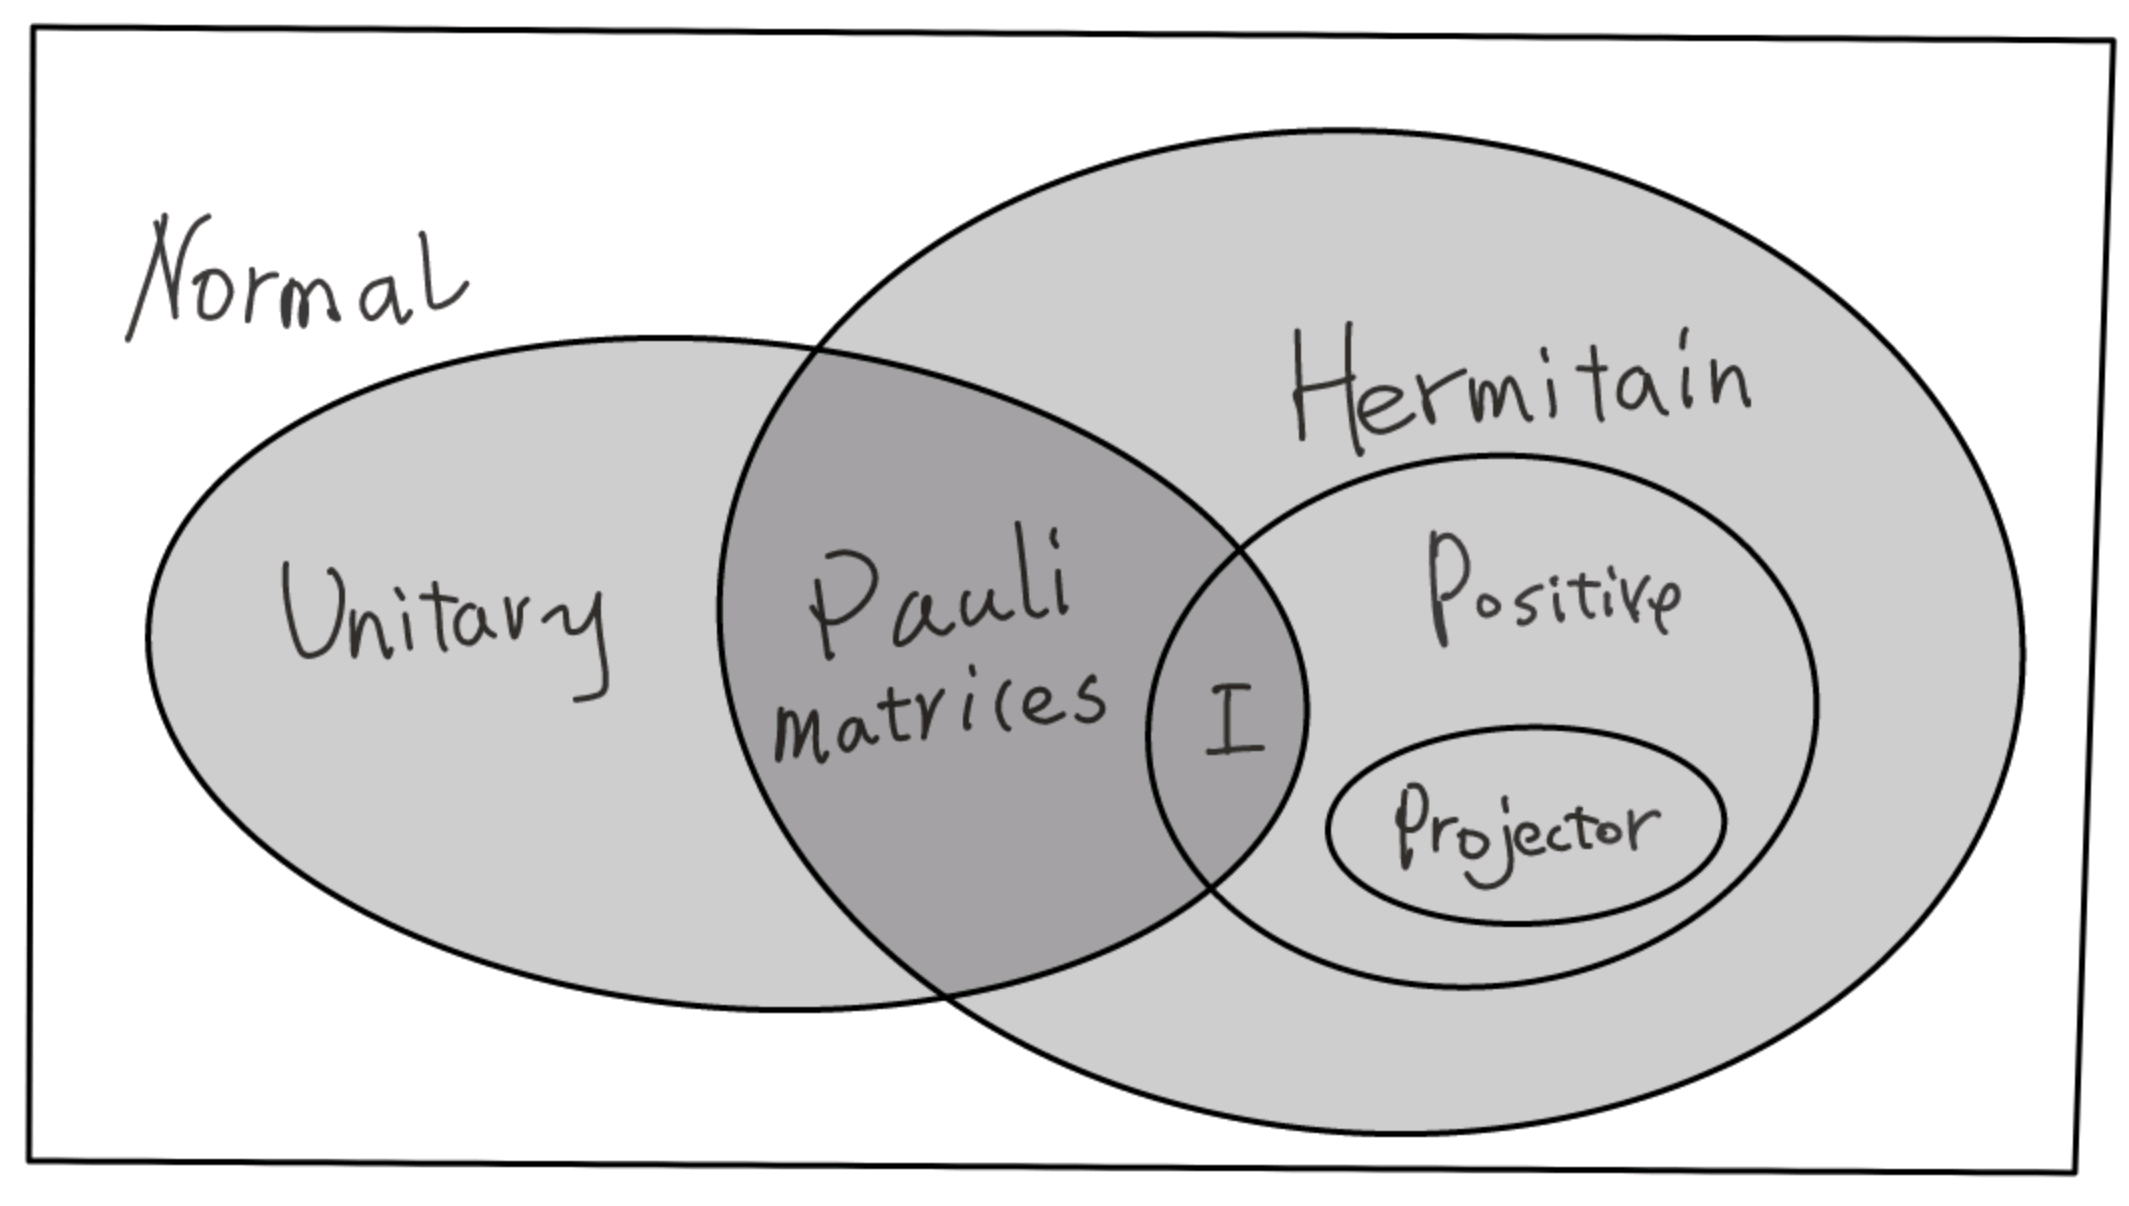
\includegraphics[width=0.75\linewidth]{Images/relations of many operators.png}
    \caption{\textbf{relations of many operators} }
\end{figure}

%   1.1.9 Tensor products
    \subsection{Tensor products}
    The tensor product is a way of putting vector spaces together to form larger vector spaces. This construction is crucial to understanding the quantum mechanics of multiparticle systems. The following discussion is a little abstract, and may be difficult to follow if you're not already familiar with the tensor product, so feel free to skip ahead now and revisit later when you come to the discussion of tensor products in quantum mechanics.

Suppose $V$ and $W$ are vector spaces of dimension $m$ and $n$ respectively. For convenience we also suppose that $V$ and $W$ are Hilbert spaces. Then $V \otimes W$ (read ' $V$ tensor

Box 2.2: The spectral decomposition - important!

The spectral decomposition is an extremely useful representation theorem for normal operators.

Theorem 2.1: (Spectral decomposition) Any normal operator $M$ on a vector space $V$ is diagonal with respect to some orthonormal basis for $V$. Conversely, any diagonalizable operator is normal.

Proof
The converse is a simple exercise, so we prove merely the forward implication, by induction on the dimension $d$ of $V$. The case $d=1$ is trivial. Let $\lambda$ be an eigenvalue of $M, P$ the projector onto the $\lambda$ eigenspace, and $Q$ the projector onto the orthogonal complement. Then $M=(P+Q) M(P+Q)=P M P+Q M P+$ $P M Q+Q M Q$. Obviously $P M P=\lambda P$. Furthermore, $Q M P=0$, as $M$ takes the subspace $P$ into itself. We claim that $P M Q=0$ also. To see this, let $|v\rangle$ be an element of the subspace $P$. Then $M M^{\dagger}|v\rangle=M^{\dagger} M|v\rangle=\lambda M^{\dagger}|v\rangle$. Thus, $M^{\dagger}|v\rangle$ has eigenvalue $\lambda$ and therefore is an element of the subspace $P$. It follows that $Q M^{\dagger} P=0$. Taking the adjoint of this equation gives $P M Q=0$. Thus $M=P M P+Q M Q$. Next, we prove that $Q M Q$ is normal. To see this, note that $Q M=Q M(P+Q)=Q M Q$, and $Q M^{\dagger}=Q M^{\dagger}(P+Q)=Q M^{\dagger} Q$. Therefore, by the normality of $M$, and the observation that $Q^{2}=Q$,

$$
\begin{aligned}
Q M Q Q M^{\dagger} Q & =Q M Q M^{\dagger} Q \\
& =Q M M^{\dagger} Q \\
& =Q M^{\dagger} M Q \\
& =Q M^{\dagger} Q M Q \\
& =Q M^{\dagger} Q Q M Q
\end{aligned}
$$

so $Q M Q$ is normal. By induction, $Q M Q$ is diagonal with respect to some orthonormal basis for the subspace $Q$, and $P M P$ is already diagonal with respect to some orthonormal basis for $P$. It follows that $M=P M P+Q M Q$ is diagonal with respect to some orthonormal basis for the total vector space.

In terms of the outer product representation, this means that $M$ can be written as $M=\sum_{i} \lambda_{i}|i\rangle\langle i|$, where $\lambda_{i}$ are the eigenvalues of $M,|i\rangle$ is an orthonormal basis for $V$, and each $|i\rangle$ an eigenvector of $M$ with eigenvalue $\lambda_{i}$. In terms of projectors, $M=\sum_{i} \lambda_{i} P_{i}$, where $\lambda_{i}$ are again the eigenvalues of $M$, and $P_{i}$ is the projector onto the $\lambda_{i}$ eigenspace of $M$. These projectors satisfy the completeness relation $\sum_{i} P_{i}=I$, and the orthonormality relation $P_{i} P_{j}=\delta_{i j} P_{i}$.

$W^{\prime}$ ) is an $m n$ dimensional vector space. The elements of $V \otimes W$ are linear combinations of 'tensor products' $|v\rangle \otimes|w\rangle$ of elements $|v\rangle$ of $V$ and $|w\rangle$ of $W$. In particular, if $|i\rangle$ and $|j\rangle$ are orthonormal bases for the spaces $V$ and $W$ then $|i\rangle \otimes|j\rangle$ is a basis for $V \otimes W$. We often use the abbreviated notations $|v\rangle|w\rangle,|v, w\rangle$ or even $|v w\rangle$ for the tensor product\\
$|v\rangle \otimes|w\rangle$. For example, if $V$ is a two-dimensional vector space with basis vectors $|0\rangle$ and $|1\rangle$ then $|0\rangle \otimes|0\rangle+|1\rangle \otimes|1\rangle$ is an element of $V \otimes V$.

By definition the tensor product satisfies the following basic properties:

(1) For an arbitrary scalar $z$ and elements $|v\rangle$ of $V$ and $|w\rangle$ of $W$,

$$
z(|v\rangle \otimes|w\rangle)=(z|v\rangle) \otimes|w\rangle=|v\rangle \otimes(z|w\rangle)
$$

(2) For arbitrary $\left|v_{1}\right\rangle$ and $\left|v_{2}\right\rangle$ in $V$ and $|w\rangle$ in $W$,

$$
\left(\left|v_{1}\right\rangle+\left|v_{2}\right\rangle\right) \otimes|w\rangle=\left|v_{1}\right\rangle \otimes|w\rangle+\left|v_{2}\right\rangle \otimes|w\rangle .
$$

(3) For arbitrary $|v\rangle$ in $V$ and $\left|w_{1}\right\rangle$ and $\left|w_{2}\right\rangle$ in $W$,

$$
|v\rangle \otimes\left(\left|w_{1}\right\rangle+\left|w_{2}\right\rangle\right)=|v\rangle \otimes\left|w_{1}\right\rangle+|v\rangle \otimes\left|w_{2}\right\rangle .
$$

What sorts of linear operators act on the space $V \otimes W$ ? Suppose $|v\rangle$ and $|w\rangle$ are vectors in $V$ and $W$, and $A$ and $B$ are linear operators on $V$ and $W$, respectively. Then we can define a linear operator $A \otimes B$ on $V \otimes W$ by the equation

$$
(A \otimes B)(|v\rangle \otimes|w\rangle) \equiv A|v\rangle \otimes B|w\rangle
$$

The definition of $A \otimes B$ is then extended to all elements of $V \otimes W$ in the natural way to ensure linearity of $A \otimes B$, that is,

$$
(A \otimes B)\left(\sum_{i} a_{i}\left|v_{i}\right\rangle \otimes\left|w_{i}\right\rangle\right) \equiv \sum_{i} a_{i} A\left|v_{i}\right\rangle \otimes B\left|w_{i}\right\rangle .
$$

It can be shown that $A \otimes B$ defined in this way is a well-defined linear operator on $V \otimes W$. This notion of the tensor product of two operators extends in the obvious way to the case where $A: V \rightarrow V^{\prime}$ and $B: W \rightarrow W^{\prime}$ map between different vector spaces. Indeed, an arbitrary linear operator $C$ mapping $V \otimes W$ to $V^{\prime} \otimes W^{\prime}$ can be represented as a linear combination of tensor products of operators mapping $V$ to $V^{\prime}$ and $W$ to $W^{\prime}$,

$$
C=\sum_{i} c_{i} A_{i} \otimes B_{i}
$$

where by definition

$$
\left(\sum_{i} c_{i} A_{i} \otimes B_{i}\right)|v\rangle \otimes|w\rangle \equiv \sum_{i} c_{i} A_{i}|v\rangle \otimes B_{i}|w\rangle .
$$

The inner products on the spaces $V$ and $W$ can be used to define a natural inner product on $V \otimes W$. Define

$$
\left(\sum_{i} a_{i}\left|v_{i}\right\rangle \otimes\left|w_{i}\right\rangle, \sum_{j} b_{j}\left|v_{j}^{\prime}\right\rangle \otimes\left|w_{j}^{\prime}\right\rangle\right) \equiv \sum_{i j} a_{i}^{*} b_{j}\left\langle v_{i} | v_{j}^{\prime}\right\rangle\left\langle w_{i} | w_{j}^{\prime}\right\rangle
$$

It can be shown that the function so defined is a well-defined inner product. From this inner product, the inner product space $V \otimes W$ inherits the other structure we are familiar with, such as notions of an adjoint, unitarity, normality, and Hermiticity.

All this discussion is rather abstract. It can be made much more concrete by moving\\
to a convenient matrix representation known as the Kronecker product. Suppose $A$ is an $m$ by $n$ matrix, and $B$ is a $p$ by $q$ matrix. Then we have the matrix representation:

$$
A \otimes B \equiv \overbrace{\left[\begin{array}{cccc}
A_{11} B & A_{12} B & \ldots & A_{1 n} B \\
A_{21} B & A_{22} B & \ldots & A_{2 n} B \\
\vdots & \vdots & \vdots & \vdots \\
A_{m 1} B & A_{m 2} B & \ldots & A_{m n} B
\end{array}\right]}^{n q} m m p
$$

In this representation terms like $A_{11} B$ denote $p$ by $q$ submatrices whose entries are proportional to $B$, with overall proportionality constant $A_{11}$. For example, the tensor product of the vectors $(1,2)$ and $(2,3)$ is the vector

$$
\left[\begin{array}{l}
1 \\
2
\end{array}\right] \otimes\left[\begin{array}{l}
2 \\
3
\end{array}\right]=\left[\begin{array}{l}
1 \times 2 \\
1 \times 3 \\
2 \times 2 \\
2 \times 3
\end{array}\right]=\left[\begin{array}{l}
2 \\
3 \\
4 \\
6
\end{array}\right]
$$

The tensor product of the Pauli matrices $X$ and $Y$ is

$$
X \otimes Y=\left[\begin{array}{cc}
0 \cdot Y & 1 \cdot Y \\
1 \cdot Y & 0 \cdot Y
\end{array}\right]=\left[\begin{array}{cccc}
0 & 0 & 0 & -i \\
0 & 0 & i & 0 \\
0 & -i & 0 & 0 \\
i & 0 & 0 & 0
\end{array}\right]
$$

Finally, we mention the useful notation $|\psi\rangle^{\otimes k}$, which means $|\psi\rangle$ tensored with itself $k$ times. For example $|\psi\rangle^{\otimes 2}=|\psi\rangle \otimes|\psi\rangle$. An analogous notation is also used for operators on tensor product spaces.

Exercise 2.26: Let $|\psi\rangle=(|0\rangle+|1\rangle) / \sqrt{2}$. Write out $|\psi\rangle^{\otimes 2}$ and $|\psi\rangle^{\otimes 3}$ explicitly, both in terms of tensor products like $|0\rangle|1\rangle$, and using the Kronecker product.

Exercise 2.27: Calculate the matrix representation of the tensor products of the Pauli operators (a) $X$ and $Z$; (b) $I$ and $X$; (c) $X$ and $I$. Is the tensor product commutative?

Exercise 2.28: Show that the transpose, complex conjugation, and adjoint operations distribute over the tensor product,

$$
(A \otimes B)^{*}=A^{*} \otimes B^{*} ;(A \otimes B)^{T}=A^{T} \otimes B^{T} ;(A \otimes B)^{\dagger}=A^{\dagger} \otimes B^{\dagger} .
$$

Exercise 2.29: Show that the tensor product of two unitary operators is unitary.

Exercise 2.30: Show that the tensor product of two Hermitian operators is Hermitian.

Exercise 2.31: Show that the tensor product of two positive operators is positive.

Exercise 2.32: Show that the tensor product of two projectors is a projector.

Exercise 2.33: The Hadamard operator on one qubit may be written as

$$
H=\frac{1}{\sqrt{2}}[(|0\rangle+|1\rangle)\langle 0|+(|0\rangle-|1\rangle)\langle 1|]
$$

Show explicitly that the Hadamard transform on $n$ qubits, $H^{\otimes n}$, may be written as

$$
H^{\otimes n}=\frac{1}{\sqrt{2^{n}}} \sum_{x, y}(-1)^{x \cdot y}|x\rangle\langle y|
$$

Write out an explicit matrix representation for $H^{\otimes 2}$.

%   1.1.10 Operator functions
    \subsection{Operator functions}
    There are many important functions which can be defined for operators and matrices. Generally speaking, given a function $f$ from the complex numbers to the complex numbers, it is possible to define a corresponding matrix function on normal matrices (or some subclass, such as the Hermitian matrices) by the following construction. Let $A=\sum_{a} a|a\rangle\langle a|$ be a spectral decomposition for a normal operator $A$. Define $f(A) \equiv \sum_{a} f(a)|a\rangle\langle a|$. A little thought shows that $f(A)$ is uniquely defined. This procedure can be used, for example, to define the square root of a positive operator, the logarithm of a positive-definite operator, or the exponential of a normal operator. As an example,

$$
\exp (\theta Z)=\left[\begin{array}{cc}
e^{\theta} & 0 \\
0 & e^{-\theta}
\end{array}\right]
$$

since $Z$ has eigenvectors $|0\rangle$ and $|1\rangle$.

Exercise 2.34: Find the square root and logarithm of the matrix

$$
\left[\begin{array}{ll}
4 & 3 \\
3 & 4
\end{array}\right]
$$

Exercise 2.35: (Exponential of the Pauli matrices) Let $\vec{v}$ be any real, three-dimensional unit vector and $\theta$ a real number. Prove that

$$
\exp (i \theta \vec{v} \cdot \vec{\sigma})=\cos (\theta) I+i \sin (\theta) \vec{v} \cdot \vec{\sigma}
$$

where $\vec{v} \cdot \vec{\sigma} \equiv \sum_{i=1}^{3} v_{i} \sigma_{i}$. This exercise is generalized in Problem 2.1 on page 117.

Another important matrix function is the trace of a matrix. The trace of $A$ is defined to be the sum of its diagonal elements,

$$
\operatorname{tr}(A) \equiv \sum_{i} A_{i i}
$$

The trace is easily seen to be cyclic, $\operatorname{tr}(A B)=\operatorname{tr}(B A)$, and linear, $\operatorname{tr}(A+B)=$ $\operatorname{tr}(A)+\operatorname{tr}(B), \operatorname{tr}(z A)=z \operatorname{tr}(A)$, where $A$ and $B$ are arbitrary matrices, and $z$ is a complex number. Furthermore, from the cyclic property it follows that the trace of a matrix is invariant under the unitary similarity transformation $A \rightarrow U A U^{\dagger}$, as $\operatorname{tr}\left(U A U^{\dagger}\right)=$ $\operatorname{tr}\left(U^{\dagger} U A\right)=\operatorname{tr}(A)$. In light of this result, it makes sense to define the trace of an operator $A$ to be the trace of any matrix representation of $A$. The invariance of the trace under unitary similarity transformations ensures that the trace of an operator is well defined.

As an example of the trace, suppose $|\psi\rangle$ is a unit vector and $A$ is an arbitrary operator. To evaluate $\operatorname{tr}(A|\psi\rangle\langle\psi|)$ use the Gram-Schmidt procedure to extend $|\psi\rangle$ to an\\
orthonormal basis $|i\rangle$ which includes $|\psi\rangle$ as the first element. Then we have

$$
\begin{aligned}
\operatorname{tr}(A|\psi\rangle\langle\psi|) & =\sum_{i}\langle i|A| \psi\rangle\langle\psi | i\rangle \\
& =\langle\psi|A| \psi\rangle
\end{aligned}
$$

This result, that $\operatorname{tr}(A|\psi\rangle\langle\psi|)=\langle\psi|A| \psi\rangle$ is extremely useful in evaluating the trace of an operator.

Exercise 2.36: Show that the Pauli matrices except for $I$ have trace zero.

Exercise 2.37: (Cyclic property of the trace) If $A$ and $B$ are two linear operators show that

$$
\operatorname{tr}(A B)=\operatorname{tr}(B A)
$$

Exercise 2.38: (Linearity of the trace) If $A$ and $B$ are two linear operators, show that

$$
\operatorname{tr}(A+B)=\operatorname{tr}(A)+\operatorname{tr}(B)
$$

and if $z$ is an arbitrary complex number show that

$$
\operatorname{tr}(z A)=z \operatorname{tr}(A)
$$

Exercise 2.39: (The Hilbert-Schmidt inner product on operators) The set $L_{V}$ of linear operators on a Hilbert space $V$ is obviously a vector space - the sum of two linear operators is a linear operator, $z A$ is a linear operator if $A$ is a linear operator and $z$ is a complex number, and there is a zero element 0 . An important additional result is that the vector space $L_{V}$ can be given a natural inner product structure, turning it into a Hilbert space.

(1) Show that the function $(\cdot, \cdot)$ on $L_{V} \times L_{V}$ defined by

$$
(A, B) \equiv \operatorname{tr}\left(A^{\dagger} B\right)
$$

is an inner product function. This inner product is known as the

Hilbert-Schmidt or trace inner product.

(2) If $V$ has $d$ dimensions show that $L_{V}$ has dimension $d^{2}$.

(3) Find an orthonormal basis of Hermitian matrices for the Hilbert space $L_{V}$.

%   1.1.11 The commutator and anti-commutator
    \subsection{The commutator and anti-commutator}
    The commutator between two operators $A$ and $B$ is defined to be

$$
[A, B] \equiv A B-B A
$$

If $[A, B]=0$, that is, $A B=B A$, then we say $A$ commutes with $B$. Similarly, the anti-commutator of two operators $A$ and $B$ is defined by

$$
\{A, B\} \equiv A B+B A
$$

we say $A$ anti-commutes with $B$ if $\{A, B\}=0$. It turns out that many important properties of pairs of operators can be deduced from their commutator and anti-commutator. Perhaps the most useful relation is the following connection between the commutator and the property of being able to simultaneously diagonalize Hermitian operators $A$ and $B$,\\
that is, write $A=\sum_{i} a_{i}|i\rangle\left\langle i\left|, B=\sum_{i} b_{i}\right| i\right\rangle\langle i|$, where $|i\rangle$ is some common orthonormal set of eigenvectors for $A$ and $B$.

Theorem 2.2: (Simultaneous diagonalization theorem) Suppose $A$ and $B$ are

Hermitian operators. Then $[A, B]=0$ if and only if there exists an orthonormal basis such that both $A$ and $B$ are diagonal with respect to that basis. We say that $A$ and $B$ are simultaneously diagonalizable in this case.

This result connects the commutator of two operators, which is often easy to compute, to the property of being simultaneously diagonalizable, which is a priori rather difficult to determine. As an example, consider that

$$
\begin{aligned}
{[X, Y] } & =\left[\begin{array}{ll}
0 & 1 \\
1 & 0
\end{array}\right]\left[\begin{array}{rr}
0 & -i \\
i & 0
\end{array}\right]-\left[\begin{array}{rr}
0 & -i \\
i & 0
\end{array}\right]\left[\begin{array}{ll}
0 & 1 \\
1 & 0
\end{array}\right] \\
& =2 i\left[\begin{array}{rr}
1 & 0 \\
0 & -1
\end{array}\right] \\
& =2 i Z
\end{aligned}
$$

so $X$ and $Y$ do not commute. You have already shown, in Exercise 2.11, that $X$ and $Y$ do not have common eigenvectors, as we expect from the simultaneous diagonalization theorem.

Proof
You can (and should!) easily verify that if $A$ and $B$ are diagonal in the same orthonormal basis then $[A, B]=0$. To show the converse, let $|a, j\rangle$ be an orthonormal basis for the eigenspace $V_{a}$ of $A$ with eigenvalue $a$; the index $j$ is used to label possible degeneracies. Note that

$$
A B|a, j\rangle=B A|a, j\rangle=a B|a, j\rangle
$$

and therefore $B|a, j\rangle$ is an element of the eigenspace $V_{a}$. Let $P_{a}$ denote the projector onto the space $V_{a}$ and define $B_{a} \equiv P_{a} B P_{a}$. It is easy to see that the restriction of $B_{a}$ to the space $V_{a}$ is Hermitian on $V_{a}$, and therefore has a spectral decomposition in terms of an orthonormal set of eigenvectors which span the space $V_{a}$. Let's call these eigenvectors $|a, b, k\rangle$, where the indices $a$ and $b$ label the eigenvalues of $A$ and $B_{a}$, and $k$ is an extra index to allow for the possibility of a degenerate $B_{a}$. Note that $B|a, b, k\rangle$ is an element of $V_{a}$, so $B|a, b, k\rangle=P_{a} B|a, b, k\rangle$. Moreover we have $P_{a}|a, b, k\rangle=|a, b, k\rangle$, so

$$
B|a, b, k\rangle=P_{a} B P_{a}|a, b, k\rangle=b|a, b, k\rangle .
$$

It follows that $|a, b, k\rangle$ is an eigenvector of $B$ with eigenvalue $b$, and therefore $|a, b, k\rangle$ is an orthonormal set of eigenvectors of both $A$ and $B$, spanning the entire vector space on which $A$ and $B$ are defined. That is, $A$ and $B$ are simultaneously diagonalizable.

Exercise 2.40: (Commutation relations for the Pauli matrices) Verify the commutation relations

$$
[X, Y]=2 i Z ; \quad[Y, Z]=2 i X ; \quad[Z, X]=2 i Y .
$$

There is an elegant way of writing this using $\epsilon_{j k l}$, the antisymmetric tensor on\\
three indices, for which $\epsilon_{j k l}=0$ except for $\epsilon_{123}=\epsilon_{231}=\epsilon_{312}=1$, and $\epsilon_{321}=\epsilon_{213}=\epsilon_{132}=-1:$

$$
\left[\sigma_{j}, \sigma_{k}\right]=2 i \sum_{l=1}^{3} \epsilon_{j k l} \sigma_{l}
$$

Exercise 2.41: (Anti-commutation relations for the Pauli matrices) Verify the anti-commutation relations

$$
\left\{\sigma_{i}, \sigma_{j}\right\}=0
$$

where $i \neq j$ are both chosen from the set $1,2,3$. Also verify that $(i=0,1,2,3)$

$$
\sigma_{i}^{2}=I
$$

Exercise 2.42: Verify that

$$
A B=\frac{[A, B]+\{A, B\}}{2}
$$

Exercise 2.43: Show that for $j, k=1,2,3$,

$$
\sigma_{j} \sigma_{k}=\delta_{j k} I+i \sum_{l=1}^{3} \epsilon_{j k l} \sigma_{l}
$$

Exercise 2.44: Suppose $[A, B]=0,\{A, B\}=0$, and $A$ is invertible. Show that $B$ must be 0 .

Exercise 2.45: Show that $[A, B]^{\dagger}=\left[B^{\dagger}, A^{\dagger}\right]$.

Exercise 2.46: Show that $[A, B]=-[B, A]$.

Exercise 2.47: Suppose $A$ and $B$ are Hermitian. Show that $i[A, B]$ is Hermitian.

%   1.1.12 The polar and singular value decomposition
    \subsection{The polar and singular value decomposition}
    The polar and singular value decompositions are useful ways of breaking linear operators up into simpler parts. In particular, these decompositions allow us to break general linear operators up into products of unitary operators and positive operators. While we don't understand the structure of general linear operators terribly well, we do understand unitary operators and positive operators in quite some detail. The polar and singular value decompositions allow us to apply this understanding to better understand general linear operators.

Theorem 2.3: (Polar decomposition) Let $A$ be a linear operator on a vector space $V$. Then there exists unitary $U$ and positive operators $J$ and $K$ such that

$$
A=U J=K U
$$

where the unique positive operators $J$ and $K$ satisfying these equations are defined by $J \equiv \sqrt{A^{\dagger} A}$ and $K \equiv \sqrt{A A^{\dagger}}$. Moreover, if $A$ is invertible then $U$ is unique.

We call the expression $A=U J$ the left polar decomposition of $A$, and $A=K U$ the right polar decomposition of $A$. Most often, we'll omit the 'right' or 'left' nomenclature, and use the term 'polar decomposition' for both expressions, with context indicating which is meant.

Proof

$J \equiv \sqrt{A^{\dagger} A}$ is a positive operator, so it can be given a spectral decomposition, $J=$ $\sum_{i} \lambda_{i}|i\rangle\langle i|\left(\lambda_{i} \geq 0\right)$. Define $\left|\psi_{i}\right\rangle \equiv A|i\rangle$. From the definition, we see that $\left\langle\psi_{i} | \psi_{i}\right\rangle=\lambda_{i}^{2}$. Consider for now only those $i$ for which $\lambda_{i} \neq 0$. For those $i$ define $\left|e_{i}\right\rangle \equiv\left|\psi_{i}\right\rangle / \lambda_{i}$, so the $\left|e_{i}\right\rangle$ are normalized. Moreover, they are orthogonal, since if $i \neq j$ then $\left\langle e_{i} | e_{j}\right\rangle=$ $\left\langle i\left|A^{\dagger} A\right| j\right\rangle / \lambda_{i} \lambda_{j}=\left\langle i\left|J^{2}\right| j\right\rangle / \lambda_{i} \lambda_{j}=0$

We have been considering $i$ such that $\lambda_{i} \neq 0$. Now use the Gram-Schmidt procedure to extend the orthonormal set $\left|e_{i}\right\rangle$ so it forms an orthonormal basis, which we also label $\left|e_{i}\right\rangle$. Define a unitary operator $U \equiv \sum_{i}\left|e_{i}\right\rangle\langle i|$. When $\lambda_{i} \neq 0$ we have $U J|i\rangle=\lambda_{i}\left|e_{i}\right\rangle=$ $\left|\psi_{i}\right\rangle=A|i\rangle$. When $\lambda_{i}=0$ we have $U J|i\rangle=0=\left|\psi_{i}\right\rangle$. We have proved that the action of $A$ and $U J$ agree on the basis $|i\rangle$, and thus that $A=U J$.

$J$ is unique, since multiplying $A=U J$ on the left by the adjoint equation $A^{\dagger}=J U^{\dagger}$ gives $J^{2}=A^{\dagger} A$, from which we see that $J=\sqrt{A^{\dagger} A}$, uniquely. A little thought shows that if $A$ is invertible, then so is $J$, so $U$ is uniquely determined by the equation $U=A J^{-1}$. The proof of the right polar decomposition follows, since $A=U J=U J U^{\dagger} U=K U$, where $K \equiv U J U^{\dagger}$ is a positive operator. Since $A A^{\dagger}=K U U^{\dagger} K=K^{2}$ we must have $K=\sqrt{A A^{\dagger}}$, as claimed.

The singular value decomposition combines the polar decomposition and the spectral theorem.

Corollary 2.4: (Singular value decomposition) Let $A$ be a square matrix. Then there exist unitary matrices $U$ and $V$, and a diagonal matrix $D$ with non-negative entries such that

$$
A=U D V
$$

The diagonal elements of $D$ are called the singular values of $A$.

Proof

By the polar decomposition, $A=S J$, for unitary $S$, and positive $J$. By the spectral theorem, $J=T D T^{\dagger}$, for unitary $T$ and diagonal $D$ with non-negative entries. Setting $U \equiv S T$ and $V \equiv T^{\dagger}$ completes the proof.

Exercise 2.48: What is the polar decomposition of a positive matrix P? Of a unitary matrix $U$ ? Of a Hermitian matrix, $H$ ?

Exercise 2.49: Express the polar decomposition of a normal matrix in the outer product representation.

Exercise 2.50: Find the left and right polar decompositions of the matrix

$$
\left[\begin{array}{ll}
1 & 0 \\
1 & 1
\end{array}\right]
$$


%   1.1.13 Partial trace
    \subsection{Partial trace}
    % 主要参考wiki
% \href{https://en.wikipedia.org/wiki/Partial_trace}{Partial trace - Wikipedia}

In linear algebra and functional analysis, the partial trace is a generalization of the trace. 
Whereas the trace is a scalar valued function on operators, the partial trace is an operator-valued function.
    
        \subsubsection{Definition with reference to a basis}
        Suppose $V, W$ are finite-dimensional vector spaces over a field, with dimensions $m$ and $n$, respectively. 
For any vector space $A$, let $L(A)$ denote the space of linear operators on $A$.

\begin{definition}[partial trace I]\label{defn:partial-trace-1}
The \textbf{partial trace over $W$} is an operator-valued function written as
$$
\operatorname{Tr}_W: \mathrm{L}(V \otimes W) \rightarrow \mathrm{L}(V),
$$
where $\otimes$ denotes the tensor product. It is defined as follows: Let $e_1, \ldots, e_m$, and $f_1, \ldots, f_n$, be bases for $V$ and $W$ respectively; then $T \in \mathrm{L}(V \otimes W)$ has a matrix representation
$$
a_{k \ell, i j}, \quad 1 \leq k, i \leq m, \quad 1 \leq \ell, j \leq n
$$
relative to the basis $e_k \otimes f_{\ell}$ of $V \otimes W$. Now fix indices $k, i$ in the range $1, \ldots, m$, consider the sum
$$
b_{k, i}=\sum_{j=1}^n a_{k j, i j}
$$
This gives a matrix $b_{k, i}$. The associated linear operator (of matrix $b_{k, i}$) on \textit{V} is independent of the choice of bases and is by definition the partial trace.
\end{definition}

Among physicists, this is often called \textbf{"tracing out" or "tracing over" $W$} to leave only an operator on $V$ in the context where $W$ and $V$ are Hilbert spaces associated with quantum systems (see below).

        \subsubsection{Definition without reference to a basis}
        The partial trace operator can be defined invariantly (that is, without reference to a basis) as follows.

\begin{definition}[partial trace II]
The \textbf{partial trace over $W$} is the unique linear map
$$
\operatorname{Tr}_W: \mathrm{L}(V \otimes W) \rightarrow \mathrm{L}(V)
$$
such that
\begin{equation}\label{eq:partial-trace-defn}
    \operatorname{Tr}_W(R \otimes S)=\operatorname{Tr}(S) R, \quad \forall R \in \mathrm{L}(V) \quad \forall S \in \mathrm{L}(W),
\end{equation}
where $\operatorname{Tr}(\cdot)$ is the usual trace of a linear operator.
\end{definition}

\begin{proof} % lai's proof
Definition \ref{defn:partial-trace-1} showed such linear map exists.
To see that the conditions (\ref{eq:partial-trace-defn}) determine the partial trace uniquely:
\begin{itemize}
  \item let $v_1, \ldots, v_m$ form an orthonormal basis for $V$ and let $w_1, \ldots, w_n$ form an orthonormal for $W$;
  \item let $E_{i j}: V \rightarrow V$ be the map that sends $v_i$ to $v_j$ (and all other basis elements to zero), then the maps $E_{i j}$ form a basis for $\mathrm{L}(V)$.
  \item let $F_{k l}: W \rightarrow W$ be the map that sends $w_k$ to $w_l$ (and all other basis elements to zero), then the maps $F_{k l}$ form a basis for $\mathrm{L}(W)$.
  \item we have $\operatorname{Tr}(E_{ij})=\operatorname{Tr}(F_{kl})=1.$
  \item since the vectors $v_i \otimes w_k$ form a basis for $V \otimes W$, the maps $E_{i j} \otimes F_{k l}$ form a basis for $\mathrm{L}(V \otimes W)$.
  \item for given \textit{any} partial trace $\operatorname{Tr}_W$, we always have that
\end{itemize}
$$
\operatorname{Tr}_W(E_{i j} \otimes F_{k l})=\operatorname{Tr}(F_{k l}) E_{i j} = E_{i j}.
$$
\end{proof}

From this abstract definition, the following properties follow:

\begin{proposition}
$$
\begin{aligned}
& \operatorname{Tr}_W\left(T\left(I_V \otimes S\right)\right)=\operatorname{Tr}_W\left(\left(I_V \otimes S\right) T\right) ,\quad \forall S \in \mathrm{L}(W) \quad \forall T \in \mathrm{L}(V \otimes W).
\end{aligned}
$$
\end{proposition}

\begin{proof}
    my proof is done on
\end{proof}

        \subsubsection{Partial trace as a quantum operation}% 待处理, 重新放在别的位置
        The partial trace can be viewed as a quantum operation.

Consider a quantum mechanical system whose state space is the tensor product $H_A \otimes H_B$ of Hilbert spaces. A mixed state is described by a density matrix $\rho$, that is a non-negative trace-class operator of trace 1 on the tensor product $H_A \otimes H_B$. The partial trace of $\rho$ with respect to the system $B$, denoted by $\rho^A$, is called the reduced state of $\rho$ on system $A$. In symbols,
$$
\rho^A=\operatorname{Tr}_B \rho
$$

To show that this is indeed a sensible way to assign a state on the $A$ subsystem to $\rho$, we offer the following justification. 

Let $M$ be an observable on the subsystem $A$, then the corresponding observable on the composite system is $M \otimes I$. However one chooses to define a reduced state $\rho^A$, there should be consistency of measurement statistics. The expectation value of $M$ after the subsystem $A$ is prepared in $\rho^A$ and that of $M \otimes I$ when the composite system is prepared in $\rho$ should be the same, i.e. the following equality should hold:
$$
\operatorname{Tr}\left(M \cdot \rho^A\right)=\operatorname{Tr}(M \otimes I \cdot \rho) .
$$
We see that this is satisfied if $\rho^A$ is as defined above via the partial trace. Furthermore, such operation is unique.

\begin{proof}
    my proof is done on
\end{proof}
    

%----------------------------------------------------------------------------------------
%	PART
%----------------------------------------------------------------------------------------

\part{Notes of Papers}

%----------------------------------------------------------------------------------------
%	PART
%----------------------------------------------------------------------------------------

\part{Other Notes}

\chapter*{Bibliography}
\markboth{\sffamily\normalsize\bfseries Bibliography}{\sffamily\normalsize\bfseries Bibliography} % Set the page headers to display a Bibliography chapter name
\addcontentsline{toc}{chapter}{\textcolor{ocre}{Bibliography}} % Add a Bibliography heading to the table of contents

\section{Articles}
\addcontentsline{toc}{section}{Articles} % Add the Articles subheading to the table of contents

\printbibliography[heading=bibempty, type=article] % Output article bibliography entries

\section{Books}
\addcontentsline{toc}{section}{Books} % Add the Books subheading to the table of contents

\printbibliography[heading=bibempty, type=book] % Output book bibliography entries

%----------------------------------------------------------------------------------------
%	INDEX
%----------------------------------------------------------------------------------------

\cleardoublepage % Make sure the index starts on an odd (right side) page
\phantomsection
\addcontentsline{toc}{chapter}{\textcolor{ocre}{Index}} % Add an Index heading to the table of contents
\printindex % Output the index

%----------------------------------------------------------------------------------------
%	APPENDICES
%----------------------------------------------------------------------------------------

\chapterimage{orange2.jpg} % Chapter heading image
\chapterspaceabove{6.75cm} % Whitespace from the top of the page to the chapter title on chapter pages
\chapterspacebelow{7.25cm} % Amount of vertical whitespace from the top margin to the start of the text on chapter pages

\begin{appendices}

\renewcommand{\chaptername}{Appendix} % Change the chapter name to Appendix, i.e. "Appendix A: Title", instead of "Chapter A: Title" in the headers

%------------------------------------------------

\chapter{Appendix Chapter Title}

\section{Appendix Section Title}

Lorem ipsum dolor sit amet, consectetur adipiscing elit. Aliquam auctor mi risus, quis tempor libero hendrerit at. Duis hendrerit placerat quam et semper. Nam ultricies metus vehicula arcu viverra, vel ullamcorper justo elementum. Pellentesque vel mi ac lectus cursus posuere et nec ex. Fusce quis mauris egestas lacus commodo venenatis. Ut at arcu lectus. Donec et urna nunc. Morbi eu nisl cursus sapien eleifend tincidunt quis quis est. Donec ut orci ex. Praesent ligula enim, ullamcorper non lorem a, ultrices volutpat dolor. Nullam at imperdiet urna. Pellentesque nec velit eget est euismod pretium.

%------------------------------------------------

\chapter{Appendix Chapter Title}

\section{Appendix Section Title}

Lorem ipsum dolor sit amet, consectetur adipiscing elit. Aliquam auctor mi risus, quis tempor libero hendrerit at. Duis hendrerit placerat quam et semper. Nam ultricies metus vehicula arcu viverra, vel ullamcorper justo elementum. Pellentesque vel mi ac lectus cursus posuere et nec ex. Fusce quis mauris egestas lacus commodo venenatis. Ut at arcu lectus. Donec et urna nunc. Morbi eu nisl cursus sapien eleifend tincidunt quis quis est. Donec ut orci ex. Praesent ligula enim, ullamcorper non lorem a, ultrices volutpat dolor. Nullam at imperdiet urna. Pellentesque nec velit eget est euismod pretium.

%------------------------------------------------

\end{appendices}

%----------------------------------------------------------------------------------------

\end{document}
